\chapter{引言}%
\label{chap:introduction}

爱因斯坦建立的广义相对论为人类理解、探索宇宙提供了必要的条件。爱因斯坦在建立
广义相对论之后不久,提出了静态宇宙解。
根据宇宙学原理的假设,弗里德曼基于Friedmann–Lemaître–Robertson–Walker (FLRW)度规,
找到了爱因斯坦场方程中的一个动态解,能够描述膨胀的宇宙。
1929年哈勃依据对河外星系退行速度的观测数据提出了哈勃定律——遥远星系的退行速度与它们和地球的距离成正比。基于观测数据的哈勃定律提出后,爱因斯坦意识到自己为了获得静态宇宙解而加入的宇宙学常数是他“一生中最大的错误”。
在弗里德曼的膨胀宇宙解以及哈勃定律的基础上,曾出现过各种非主流宇宙模型。
到了40年代,出现了热大爆炸理论,预言了轻元素丰度、宇宙微波背景辐射。后来原初核合成理论的成功以及1964年宇宙微波背景辐射的发现和确认强烈支持热大爆炸理论。
尽管热大爆炸理论能很好地解释宇宙膨胀、宇宙微波背景辐射、大尺度结构以及物质起源
等问题,但仍然存在一些疑难无法解释,例如视界问题、平坦性问题、磁单极问题等等。
为了解决这些问题,Guth在1981年首次提出了暴涨的概念,认为宇宙早期应该存在一个
短暂的加速膨胀过程,膨胀结束之后直到当前时刻则能用热大爆炸理论进行描述。在暴涨
过程开始之前,目前的整个可观测区域均处在一个均匀且各项同性的区域内。随后在暴涨
的作用下,这块区域开始加速膨胀。膨胀的速度是如此之快,以至于暴涨结束之后,
这块区域的尺度远远超过了当时的哈勃尺度。

后来关于星系旋转曲线的观测数据以及其它一些实验暗示宇宙中应当存在某种不参与
电磁相互作用的物质,被称为暗物质。另外有一些天文观测表明除了暗物质,
应当还有暗能量存在,例如暗物质与普通物质的观测总量远小于大爆炸理论中的临界密度
,然而实际观测却支持宇宙是平坦的。热大爆炸理论、暗物质、暗能量以及暴涨模型
共同组成了目前广为接受的标准宇宙学模型,包含六个基本参数。
标准宇宙学模型对宇宙演化的描述基本如图$(\ref{fig:history-of-universe})$所描述的样子。

\begin{figure*}[!htbp]
  \centering
  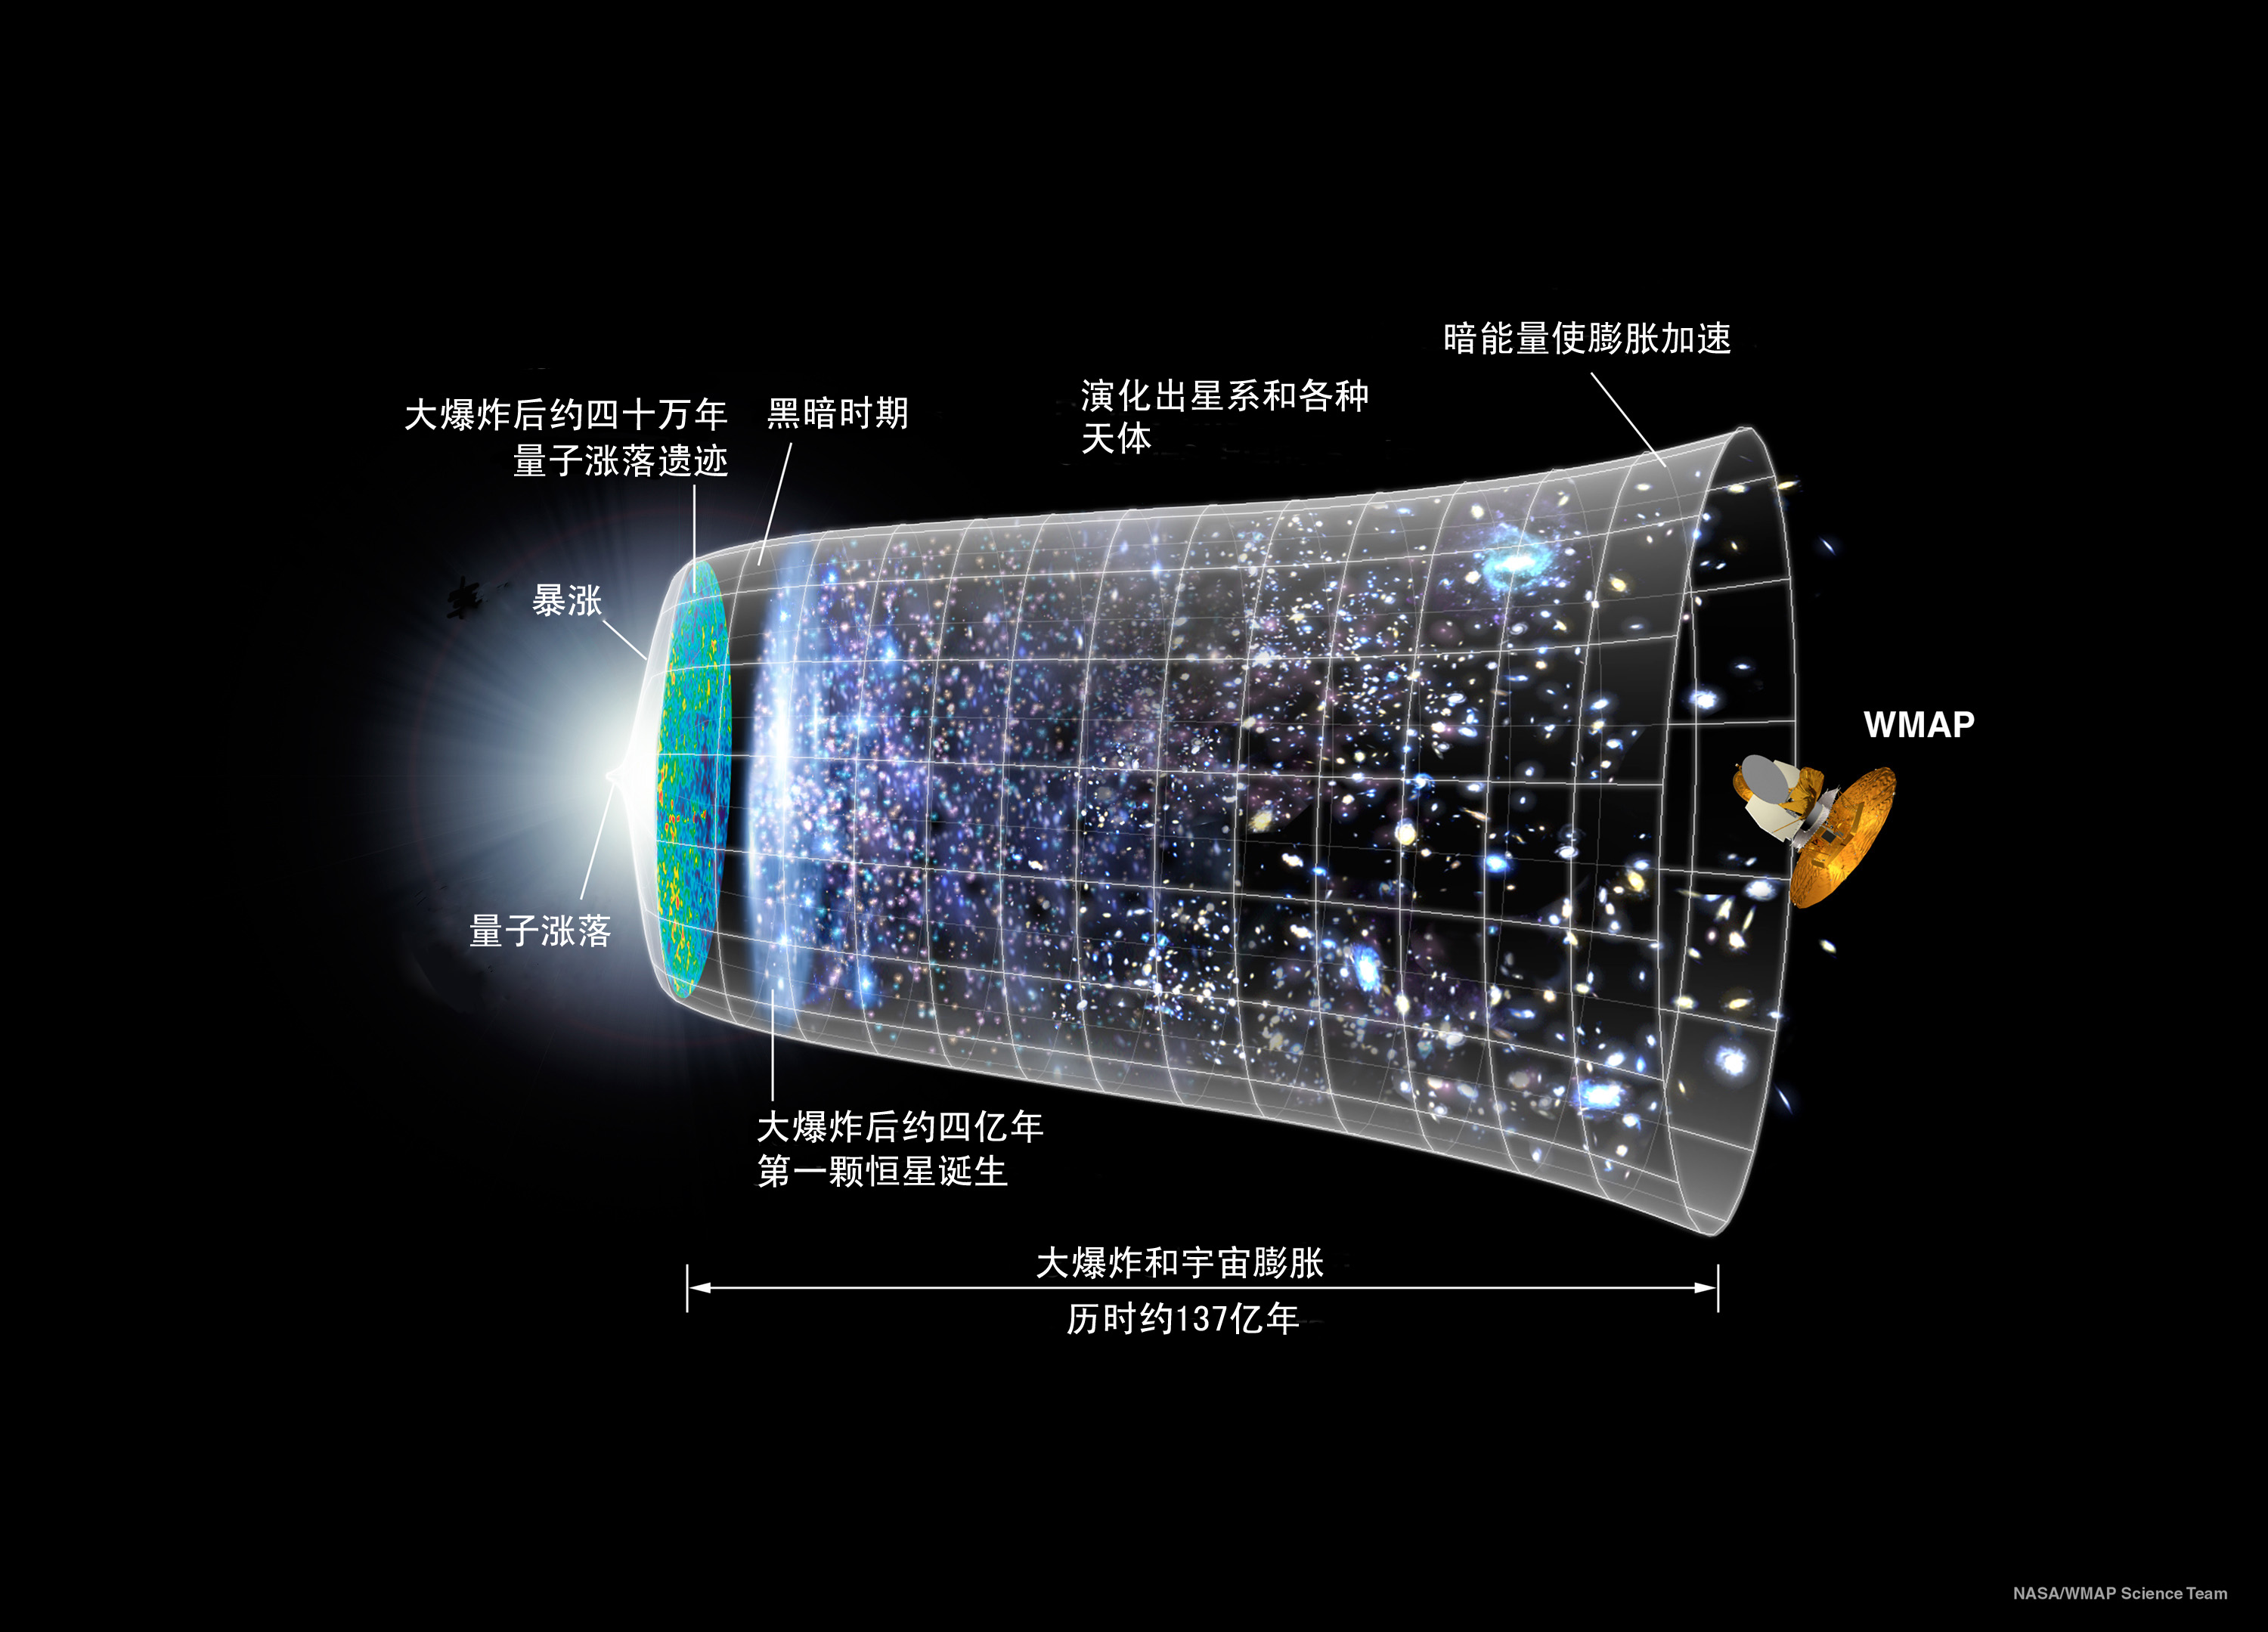
\includegraphics[width=6in]{Img/CMB_Timeline75_zh-cnversion.jpg}
  \caption{宇宙演化,图片来自2006年WMAP新闻发布会。}\label{fig:history-of-universe}
\end{figure*}


暴涨理论提供了一种产生原初扰动的机制,产生的标量扰动和张量扰动以一种自然的方式
解释了CMB中观测到的各项异性以及提供了宇宙大尺度结构能够形成的种子。其中标量扰动
的存在已经被CMB各项异性的观测所看到\citep{akrami2018planck}。
大尺度上的张量扰动虽然还未被观测到,但是Planck
2018联合BICEP2/Keck阵列的数据对张标比$r$的上限给出了更紧的限制,在$95\%$的置信水平上$r<0.064$。

线性扰动理论中,张量扰动满足的演化方程是无源的波动方程。而在二阶扰动的情况下,自由波动方程获得了一个来自标量扰动的源项\citep{matarrese1998relativistic,acquaviva2002second}。标量扰动在辐射为主时期进入哈勃视界后能够诱导产生引力波。
如果假设标量扰动的功率谱函数是幂指数形式,那么与暴涨期间产生的无源引力波相比,
诱导引力波完全可以被忽略\citep{ananda2007cosmological,baumann2007gravitational},因为根据Planck
2018年的数据,标量谱指标$n_{s}$在$68\%$的置信水平上被限制在$n_{s}=0.9649\pm 0.0042$。
但假若标量功率谱在小尺度上有一个加强的话,诱导引力波的强度甚至可以增大到可以与
一阶引力波相比拟,届时便必须考虑它的影响\citep{assadullahi2009gravitational,alabidi2013observable,alabidi2012observable,chen2019pulsar,cai2019gravitational,inomata2019gravitational,cai2019universal}。并且小尺度上功率谱的增强会使得扰动在辐射为主时期进入视界后通过引力塌缩的方式生成原初黑洞\citep{garcia1996density,clesse2015massive,yokoyama1995formation,dalianis2019primordial,gao2018primordial,di2018primordial,garcia2017primordial,garcia2016gravitational}。
因此标量扰动诱导产生的引力波可以用来约束原初黑洞的丰度,反过来原初黑洞的丰度也能用于限制诱导引力波的性质。

尽管已有大量的暴涨模型被提出,但是关于暴涨的理论起源依然是一个开放的课题。因此
如何从更基本的理论出发构造与观测相一致的暴涨模型是一个重要的课题。
我们的第一个工作就是在超引力的框架内实现了拐点暴涨模型,预言了与CMB观测一致的功率谱。

此前已经有工作\citep{garcia1702phys}通过单拐点的单场暴涨模型成功使标量谱在小尺度上得到增强。其中用到的拐点暴涨模型是在超引力框架内利用对数K\"ahler势和三次方超势构造得来\citep{gao2015inflection}。
近期,又有文章在超引力中基于单手征超场构造出了双拐点暴涨模型\citep{gao2018primordial},
其中一个拐点在大尺度上生成与CMB相一致的功率谱,
另一个拐点使得功率谱在小尺度上产生一个峰。这个峰的存在使得扰动在辐射为主时期进入视界后能够产生原初黑洞。
基于这个背景,产生了我们的第二个工作。在\citep{gao2018primordial}中双拐点暴涨模型的基础上
用解析方法计算诱导引力波的大小,并与LISA和太极的观测灵敏度进行比较,看诱导引力波的信号是否有可能被探测到。

文章的结构如下:

第二章介绍暴涨宇宙学,包括四个部分。
第一部分介绍标准宇宙学模型,从宇宙热大爆炸理论到$\Lambda$CDM模型。
第二部分介绍暴涨宇宙学,包括暴胀模型提出的动机、思想及理论。
第三部分介绍宇宙扰动理论,包括扰动的分解、规范变换以及演化方程。第四部分推导
标量扰动和张量扰动的原初功率谱。

第三章介绍超引力框架下的拐点暴涨模型,包括三个部分。
第一部分简单介绍了基于超引力的暴涨理论的历史,包括超引力暴涨模型发展过程中遇到的一些问题以及解决方法。
第二部分介绍了跑动动能暴涨模型,包含跑动动能暴涨模型提出的背景,以及这一类暴涨模型的基本特点。
第三部分我们在超引力框架下,
通过选取超势$W$,并对参数进行微调得到了具有拐点的暴涨势。并以
Planck 2015
数据中曲率扰动的大小作为约束条件,计算了多种参数取值下的$n_{s}-r$的预测值,
并将其与 Planck 2015 数据进行了比较,发现与观测较为符合。

第四章介绍了双拐点暴涨模型预言的随机引力波背景,包括四个部分。
第一部分介绍了双拐点暴涨模型,及其特点。
第二部分首先介绍了超引力下的单场暴涨模型,
然后通过选取满足约束条件的超势构造了一个单场暴涨模型,并且在暴涨结束会得到一个恢复超对称的闵可夫斯基真空。进一步在参数空间中调节超势中引入的几个参数值,将构造出
具有双拐点的暴涨模型。
第三部分给出了所构造的双拐点暴涨模型对应的功率谱,由于拐点的
存在,包含慢滚参数的计算功率谱的近似公式将不再适用,因而采用数值方法求解MS方程。
% 第四部分简单介绍原初黑洞,根据原初洞的生成机制以及观测数据,调节功率谱中峰的位置以及幅度。
第四部分我们数值计算了标量扰动诱导引力波的能谱,并将其与LISA\citep{amaro2017laser}和太极\citep{guo2018taiji}的观测灵敏度曲线进行比较。对功率谱进行函数拟合后,对得到的结果进行了一定的推广讨论。

最后一章是总结与展望。
